\documentclass[12pt,a4paper]{article}
\usepackage[UTF8]{ctex}
\usepackage{amsmath,amssymb}
\usepackage{listings}
\usepackage{xcolor}
\usepackage{hyperref}
\usepackage{geometry}
\usepackage{graphicx}
\geometry{margin=2.5cm}

\lstdefinestyle{python}{
  language=Python,
  basicstyle=\ttfamily\small,
  keywordstyle=\color{blue}\bfseries,
  commentstyle=\color{gray},
  stringstyle=\color{red},
  showstringspaces=false,
  breaklines=true,
  frame=single,
  backgroundcolor=\color{gray!10}
}

\title{Quantum Walk / 量子行走}
\author{QuoNic}
\date{}

\begin{document}
\maketitle

\begin{center}
\textbf{Algorithms / 算法} | 难度：中级 | 预计时间：15 分钟
\end{center}

\tableofcontents
\newpage

\section{为什么需要？}

量子行走是经典随机行走的量子推广，是许多量子算法的基础。

\subsection{经典局限}
\b\begin{itemize}
  \item 经典随机行走：扩散速度 $O(\sqrt{t})$
  \item 经典行走需要 $O(t)$ 时间到达距离 $t$
\end{itemize}

\subsection{量子优势}
\b\begin{itemize}
  \item 量子行走：扩散速度 $O(t)$
  \item 量子行走提供二次加速
  \item 是许多量子算法的基础（搜索、图算法）
\end{itemize}

\subsection{实际应用}
\b\begin{itemize}
  \item 图搜索（二次加速）
  \item 图同构问题
  \item 量子算法设计
\end{itemize}

\section{快速上手}

\begin{lstlisting}[style=python]
from quonic.algorithms import quantum_walk

# Quantum walk on a line
result = quantum_walk(steps=10, graph="line")
print(f"Position distribution: {result.distribution}")
\end{lstlisting}

\textbf{预期输出}：
\begin{verbatim}
Position distribution: {0: 0.1, 2: 0.2, 4: 0.3, ...}
\end{verbatim}

\section{原理详解}

\subsection{电路图}

\begin{center}
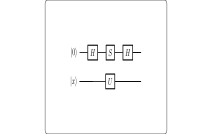
\includegraphics[width=0.6\textwidth]{../../images/quantum_walk_circuit.svg}
\end{center}

\subsection{数学推导}

量子行走的演化算子：
\begin{equation}
U = S \cdot (H \otimes I)
\end{equation}

其中 $S$ 是条件移位算子，$H$ 是 Hadamard 门。

\textbf{一步行走}：
\begin{equation}
|\psi_{t+1}\rangle = U|\psi_t\rangle
\end{equation}

\subsection{几何解释}

量子行走利用量子叠加态同时探索多个路径，通过干涉效应实现二次加速。

\section{代码详解}

\begin{lstlisting}[style=python]
from quonic.algorithms import quantum_walk

# quantum_walk(steps, graph, shots)
# steps: number of walk steps
# graph: graph type (line, cycle, complete)
# shots: number of measurements
result = quantum_walk(steps=10, graph="line", shots=1024)

# result.distribution: position probability distribution
# result.positions: measured positions
print(f"Distribution: {result.distribution}")
\end{lstlisting}

\section{进阶用法}

\subsection{场景 1：不同图}

\begin{lstlisting}[style=python]
# Walk on different graphs
result_line = quantum_walk(steps=10, graph="line")
result_cycle = quantum_walk(steps=10, graph="cycle")
result_complete = quantum_walk(steps=10, graph="complete")
\end{lstlisting}

\subsection{场景 2：不同步数}

\begin{lstlisting}[style=python]
# Different number of steps
for steps in [5, 10, 20, 50]:
    result = quantum_walk(steps=steps, graph="line")
    print(f"Steps: {steps}, Spread: {result.spread}")
\end{lstlisting}

\section{适用场景}

\subsection{图搜索}

量子行走可以用于图搜索，提供二次加速。

\subsection{图算法}

量子行走可以用于图同构、图连通性等问题。

\subsection{量子算法设计}

量子行走是许多量子算法的基础。

\section{常见问题}

\subsection{量子行走和经典随机行走有什么区别？}

量子行走利用量子叠加和干涉，扩散速度是经典的平方。

\subsection{量子行走需要多少量子比特？}

量子行走需要的量子比特数取决于图的大小。

\section{学习路径}

\subsection{前置知识}
\b\begin{itemize}
  \item 量子比特和量子门
  \item Hadamard 门
  \item 量子测量
\end{itemize}

\subsection{继续学习}
\b\begin{itemize}
  \item 量子搜索算法
  \item 量子图算法
  \item 量子模拟
\end{itemize}

\section{完整示例代码}

\subsection{示例 1：基本量子行走}

\begin{lstlisting}[style=python]
from quonic.algorithms import quantum_walk

result = quantum_walk(steps=10, graph="line")
print(f"Distribution: {result.distribution}")
\end{lstlisting}

\

\section{下载}

\begin{itemize}
  \item [quantum_walk.py](https://github.com/ChrisLee0721/QuoNic/blob/main/examples/quantum_walk/quantum_walk.py)
\end{itemize}

\end{document}
